\chapter{Literature Review}

\section{Cut-off}

A scorecard in simple terms is just a method producing a score for each individual. To put the scorecard into use the difference between the scores needs to be classified this is done by a cut-off score. This score is a point on the scorecard which would seperate accepted applicants from rejected. A simple cut-off method would be to have a single score, any applicants above the score are accepted and anyone below the score is rejected. The benefit of a simple method is the ability to quickly process applicants and move desired applicants onto the next stage faster. The issue with the single cutoff comes with the applicants that are close to the cutoff, having a strict cut-off can cause a company to take on bad applicants or reject good applicants where futher investigation would prove the applicant more likely to be the opposite. \\

An alternative to this would be a two score cut-off. This would be done by having two scores like $ \textup{Rejected } < S_{1} < \textup{ Refer } < S_{2} < \textup{ Accepted}$. Any score above $S_{2}$ is automatically accepted and any below $S_{1}$ is rejected. Scores which the land in between and moved to a referral stage where a lender can further look into the applicants case by case to decide the outcome. This comes with added benefit of removing the issue of applicants close to the single cutoff. The idea is that with the lenders insight, more good applicants will be accepted and more bads rejected compared to the single cutoff, thus possibly reducing the bad rate of accepted applicants. \\

The cut-off scores can be determined by varying factors which can change depending on the companies interest. Four of these are specified by \parencite{bailey2004credit}. Acceptance rate, the percentage of all applicants accepted by the cut-off. Overall bad rate, the percentage of all accepted applicants that end up being bads. Marginal bad rate, the percentage of accepted applicancts that are bad close to the cut-off score. Profitability, the possible profit from goods minus the loss from bads. Depending on the situation of the business and its goals would determine the importance of each factor with overal bad rate being the usual priority.

\section{Weight of evidence and Information value}  \label{sec:woe_and_iv}

Weight of evidence, WOE. Is a popular method used in score card modelling, often used because the variables used in credit scoring can have a large amount of categories which cause impractiallities when converting these to dummy variables. WOE is an alternative to that, rather than creating a large amount of dummy variables, the method produces a numerical value (weight of evidence) for each category/bin which is prdouced by Equation (\ref{WOE}). These values would then replace their respective categorical/bin value before using whichever modelling method used to develop the scorecard.

\begin{equation}\label{WOE}
WOE = \ln \frac{f(X=x|y=0)}{f(X=x|y=1)}
\end{equation}

where $f()$ is the distribution of category $X$ for either goods $(y=0)$ or bads $(y=1)$. \\

The information value, IV. Is a measure of the weight of evidence for categories $IV \geq 0$. A value of 0 indicates the variable has no predictive power i.e. no valuable information in the variable. IV can be calculated by Equation (\ref{IV}). A guideline produced by \parencite{bailey2004credit} is below for evaluating the IV values.

\begin{equation}\label{IV}
\textup{IV} = \sum (\% \textup{ of Bad} - \% \textup{ of Good}) \cdot \textup{WOE}
\end{equation}

\begin{table}[H]
	\centering
	\begin{tabular}{l l l l}
	IV	&Recommendation \\
	\hline
	Less than 0.03			&Poor Predictor \\
	From 0.03 to less than 0.10	&Weak Predictor \\
	From 0.10 to less than 0.30	&Average Predictor \\
	From 0.30 to less than 0.50	&Strong Predictor \\
	Over 0.50				&Very Strong Predictor \\
	\end{tabular}
	\caption{Information Value Table \label{IV}}\parencite{bailey2004credit}
\end{table}

\section{Performance Evaulation} \label{sec:perf_eval}

\subsection*{ROC and AUC}
ROC, Receiver Operating Characteristic. Was a method of analysis developed during World War II under "Signal Detection Theory". It was originally used for radar operators and their ability to determine if a blip on screen was an enemy or just noise, hence the name Receiver Operating Characteristics \parencite{tape2000using}. Since then, the method has been applied into a variety of fields for visuallising the accuary of classification models. \\

Understanding the ROC Curve is relatively simple, the plot is the false positive rate against true positive rate for different cutoff points. The true positive rate is seen as the sensitivity and the false positive being (1 - specificity) An example figure can be found below, the higher the curve, the more accurate the model can be seen as, with the neutral line going 45 degrees through the plot can be seen as the model being the same as a 50/50 guess on the outcome. In some cases these curves can overlap and cause some ambiguity on which curve is overall the best so the measure used to remove this amiguity is the AUC, Area under the curve (\ref{AUC}). A higher AUC inidicates a stronger disciminatory power with 0.5 being none and 1 being a "perfect model". As such the model with a higher AUC can be considered "a better model". Generally, an $AUC > 0.8$ is considerd good.

\begin{equation}\label{AUC}
A = \int_{c}^{} F_1(c){F_0}'(c) dc
\end{equation}

A more common representation of the AUC is the gini coefficient (\ref{GINI}). A linear transformation of the AUC to allow the measure to have a preferred 0 to 1 scale rather than 0.5 to 1.

\begin{equation}\label{GINI}
gini = (2 \cdot AUC) - 1
\end{equation}

\begin{figure}[!ht]
	\centering
	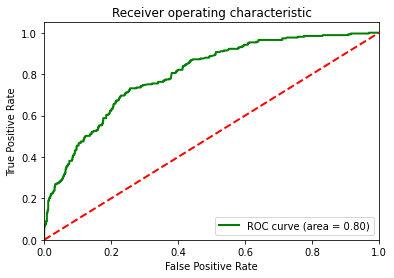
\includegraphics[scale=1.00]{figs/roc_example.png}
	\caption{ROC Example \label{roc_example}}
\end{figure}

\subsection*{K-S Statistic}

The K-S Statistic (Kolmogorov-Smirnov Statistic) is a measurement of the scorecards ability to seperate the goods from bads. The K-S Statistic is the maximum distance between the cumulative distributions of both the goods and bads, or alterntively, if $F_{g}(x)$ is the cumulative distribution of goods and bads is $F_{b}(x)$ where $x$ is the score then the K-S Statistic is (\ref{KS})

\begin{equation}\label{KS}
KS = max(F_{g}(x) - F_{b}(x))
\end{equation}

An issue of this measurement is that it only provides the score at which the scordcard seperates the goods and bads the most. The cutoff score for the card might not necessarily be this score and a higher K-S score does not imply the scorecard is a better fit. 

\subsection*{Divergence}

Divergence is a measurement of the distributions of goods and bads. The idea is that the scorecard on average will assign a lower score to bads than goods i.e. $\mu_{b} < \mu_{g}$. Divergence is a way to assess this performance. Specified by \parencite{bailey2004credit} divergence is calculated by Equation (\ref{eq:divergence})

\begin{equation}\label{eq:divergence}
Divergence = \dfrac{(\mu_g - \mu_b)^2}{\dfrac{1}{2} (\sigma_g^2 + \sigma_b^2)}
\end{equation}

Where $\mu$ is the mean and $\sigma^2$ is the variance and g and b are goods and bads respectively

\subsection*{Population Stability Index}

The population stability index, PSI. Is a measure of the distributions of two populations to ensure similarity. Credit score models are developed using historical data and it is important to ensure that the data used to model the scorecard does not differ too much from the data the model will be used to assess. A high PSI can result in investigation as the use of the model could potentially be unsuitable and cause an increase in risk from the company \parencite{yurdakul2018statistical}. Although the data being used is collected in the same time period, PSI can still be used to compare train and test data sets to ensure there isn't a large population shift between the two.\\

Interpretation of the PSI in the industry is not set in stone. The general guideline mentioned by \parencite{bailey2004credit} is that a psi of less than 10\% indicates no shift, 10 to 25\% shows a slight shift and should be investiaged and a PSI greater than 25\% suggests the model should be revaluated on more recent data. PSI can be calculated using the Equation (\ref{eq:psi})\parencite{yurdakul2018statistical}.

\begin{equation}\label{eq:psi}
PSI = \sum_{i=1}^{B} (y_i-y_{b_i}) * ln(\dfrac{y_i}{y_{b_i}})
\end{equation}

where $y_i$ is the proportion of target year credit scores that fall in the ith bin, $y_{b_i}$ is the proportion of base year credit scores than fall in the ith bin and B represents the number of bins.

\section{Data Cleaning Methods}

Missing data is a problem that comes with any raw dataset that you might come across and there are a variety of methods to handelling them. Missing data can be categorised into 3 types, missing completely at random, MCAR. Missing at random, MAR, and missing not at random, MNAR. The most common assumption is that the data is MAR, missing data is not missing because of the value but rather a function from some other observered variable. (e.g. an applicant with category A may not want to disclose the value of the variable where as an applicant in category B is more likely to disclose). MCAR is when the probability of missingness is unreleated to the observed variables such as a study participant not returning for a follow-up, etc. MNAR is when the variable is missing due to the value of the variable, for example someone may not want to disclose their income if they consider it to be on the lower end \parencite{buhi2008out}. Determining what category the variable lies in is often impossible in practice as to determine if a variable is MNAR you would need to know what those missing values are to compare with the values not missing which is often not available \parencite{newman2014missing}.\\

For this project I decide to use a mixture of data cleaning methods, regression imputation, single imputation and listwise deletion. Regression imputation is the use of other available data to develop a regression model to predict the missing values. Single imputation is the use of the available data from the variable and impute the same value for each, e.g. the use of mean, median, mode as the value for the remaining. Listwise deletion is the removal of any observation with missing data remaining.

\section{Chimerge Discretization} \label{chimerge}

For the application of the woe methods a python package called scorecardpy will be used to help automate the process by finding the optimal bins for the numerical variables. The package has the two options for optimizing, tree based and chimerge. For this project I will be using the chimerge method and will explain its application. \\

The chimerge methods uses the $\chi^2$ statistic to bin numerical variables. It can be seen in detail in \parencite{kerber1992chimerge}. The intial step is for the variables to be sorted and then each observation will be split into it's own bin. Each bin will then be compared to its adjacent and calculate the $\chi^2$ value, the bin is then merged into the adjcent bin with the lowest $\chi^2$ value. This step is repeated until all pairs have $\chi^2$ values exceeding a threshold. The formula for computing $\chi^2$ can be seen in Equation (\ref{CHI}).

\begin{equation}\label{CHI}
\chi^2 = \sum^{m}_{i=1}\sum^{k}_{j=1} \dfrac{(A_{ij} - E_{ij})^2}{ E_{ij}}
\end{equation}

where, m = 2, the two intervals being compared. k is the number of classes, in our case 2 (Good and Bad). $A_{ij}$ is the number of observations in ith interval and jth class. $E_{ij}$ is the expected frequency of $A_{ij}$ which is calculated by Equation (\ref{AFREQ}).

\begin{equation}\label{AFREQ}
A_{ij} = \dfrac{R_i - C_j}{N}
\end{equation}

where, $R_i$ is the number of observations in ith interval. $C_j$ is the number of observations in jth class and N is the total number of observations.

